\chapter{Database Data Dictionary}

\section{Overview}
A robust relational database relies on strict data typing, foreign key constraints, and indexing. This appendix serves as the comprehensive Data Dictionary for the Kemora SQL Server database, detailing the exact schema generated by the Entity Framework Core migrations.

\section{Table: ApplicationUsers}
Stores the core identity and gamification metrics for authenticated users.
\begin{longtable}{|l|l|p{6cm}|}
\hline
\textbf{Column Name} & \textbf{Data Type} & \textbf{Description / Constraints} \\ \hline
Id & NVARCHAR(450) & Primary Key. Generated UUID (Inherited from IdentityUser). \\ \hline
UserName & NVARCHAR(256) & Nullable. User's chosen username (Inherited). \\ \hline
NormalizedUserName & NVARCHAR(256) & Nullable. Uppercase username for fast lookups (Inherited). \\ \hline
Email & NVARCHAR(256) & Unique Index. User's login email (Inherited). \\ \hline
NormalizedEmail & NVARCHAR(256) & Nullable. Uppercase email (Inherited). \\ \hline
EmailConfirmed & BIT & Required. Indicates if email is verified (Inherited). \\ \hline
PasswordHash & NVARCHAR(MAX) & Nullable. PBKDF2 hashed password string (ASP.NET Core Identity default, inherited). \\ \hline
SecurityStamp & NVARCHAR(MAX) & Nullable. Value that changes on credential change (Inherited). \\ \hline
ConcurrencyStamp & NVARCHAR(MAX) & Nullable. Concurrency token (Inherited). \\ \hline
PhoneNumber & NVARCHAR(MAX) & Nullable. User's phone number (Inherited). \\ \hline
PhoneNumberConfirmed & BIT & Required. Indicates if phone is verified (Inherited). \\ \hline
TwoFactorEnabled & BIT & Required. Indicates if 2FA is enabled (Inherited). \\ \hline
LockoutEnd & DATETIMEOFFSET & Nullable. When the lockout ends (Inherited). \\ \hline
LockoutEnabled & BIT & Required. Indicates if user can be locked out (Inherited). \\ \hline
AccessFailedCount & INT & Required. Number of failed login attempts (Inherited). \\ \hline
FullName & NVARCHAR(MAX) & Required. User's display name. \\ \hline
ProfilePictureUrl & NVARCHAR(MAX) & Nullable. \\ \hline
Bio & NVARCHAR(MAX) & Nullable. \\ \hline
Country & NVARCHAR(MAX) & Required. User's country of origin. \\ \hline
TotalPoints & INT & Default: 0. Aggregated gamification score. \\ \hline
RefreshToken & NVARCHAR(MAX) & Nullable. Used for issuing new JWTs without re-login. \\ \hline
RefreshTokenExpiryTime & DATETIME2 & Required. Timestamp of token expiration. \\ \hline
UserPreferencesJSON & NVARCHAR(MAX) & Nullable. Stores Budget, Vibe, Pace etc. \\ \hline
\caption{ApplicationUsers Table Schema}
\end{longtable}

\section{Table: Badges}
Stores gamification badges that users can earn.
\begin{longtable}{|l|l|p{6cm}|}
\hline
\textbf{Column Name} & \textbf{Data Type} & \textbf{Description / Constraints} \\ \hline
BadgeID & INT & Primary Key. Auto-incremented. \\ \hline
Name & NVARCHAR(MAX) & Required. \\ \hline
Description & NVARCHAR(MAX) & Required. \\ \hline
IconUrl & NVARCHAR(MAX) & Required. \\ \hline
Criteria & NVARCHAR(MAX) & Required. \\ \hline
PointsReward & INT & Required. \\ \hline
\caption{Badges Table Schema}
\end{longtable}

\section{Table: UserBadges}
Mapping table between users and the badges they have earned.
\begin{longtable}{|l|l|p{6cm}|}
\hline
\textbf{Column Name} & \textbf{Data Type} & \textbf{Description / Constraints} \\ \hline
UserID & NVARCHAR(450) & Composite Key component / Foreign Key $\rightarrow$ ApplicationUsers(Id). \\ \hline
BadgeID & INT & Composite Key component / Foreign Key $\rightarrow$ Badges(BadgeID). \\ \hline
EarnedAt & DATETIME2 & Required. Timestamp of when the badge was earned. \\ \hline
\caption{UserBadges Table Schema}
\end{longtable}

For the full data dictionary encompassing all entities, please refer to the project's GitHub repository.

\section{Database Entity Relationship Diagram (ERD)}
Below is the visual representation of the Kemora database schema, illustrating the core entities and their relationships.

\begin{figure}[H]
    \centering
    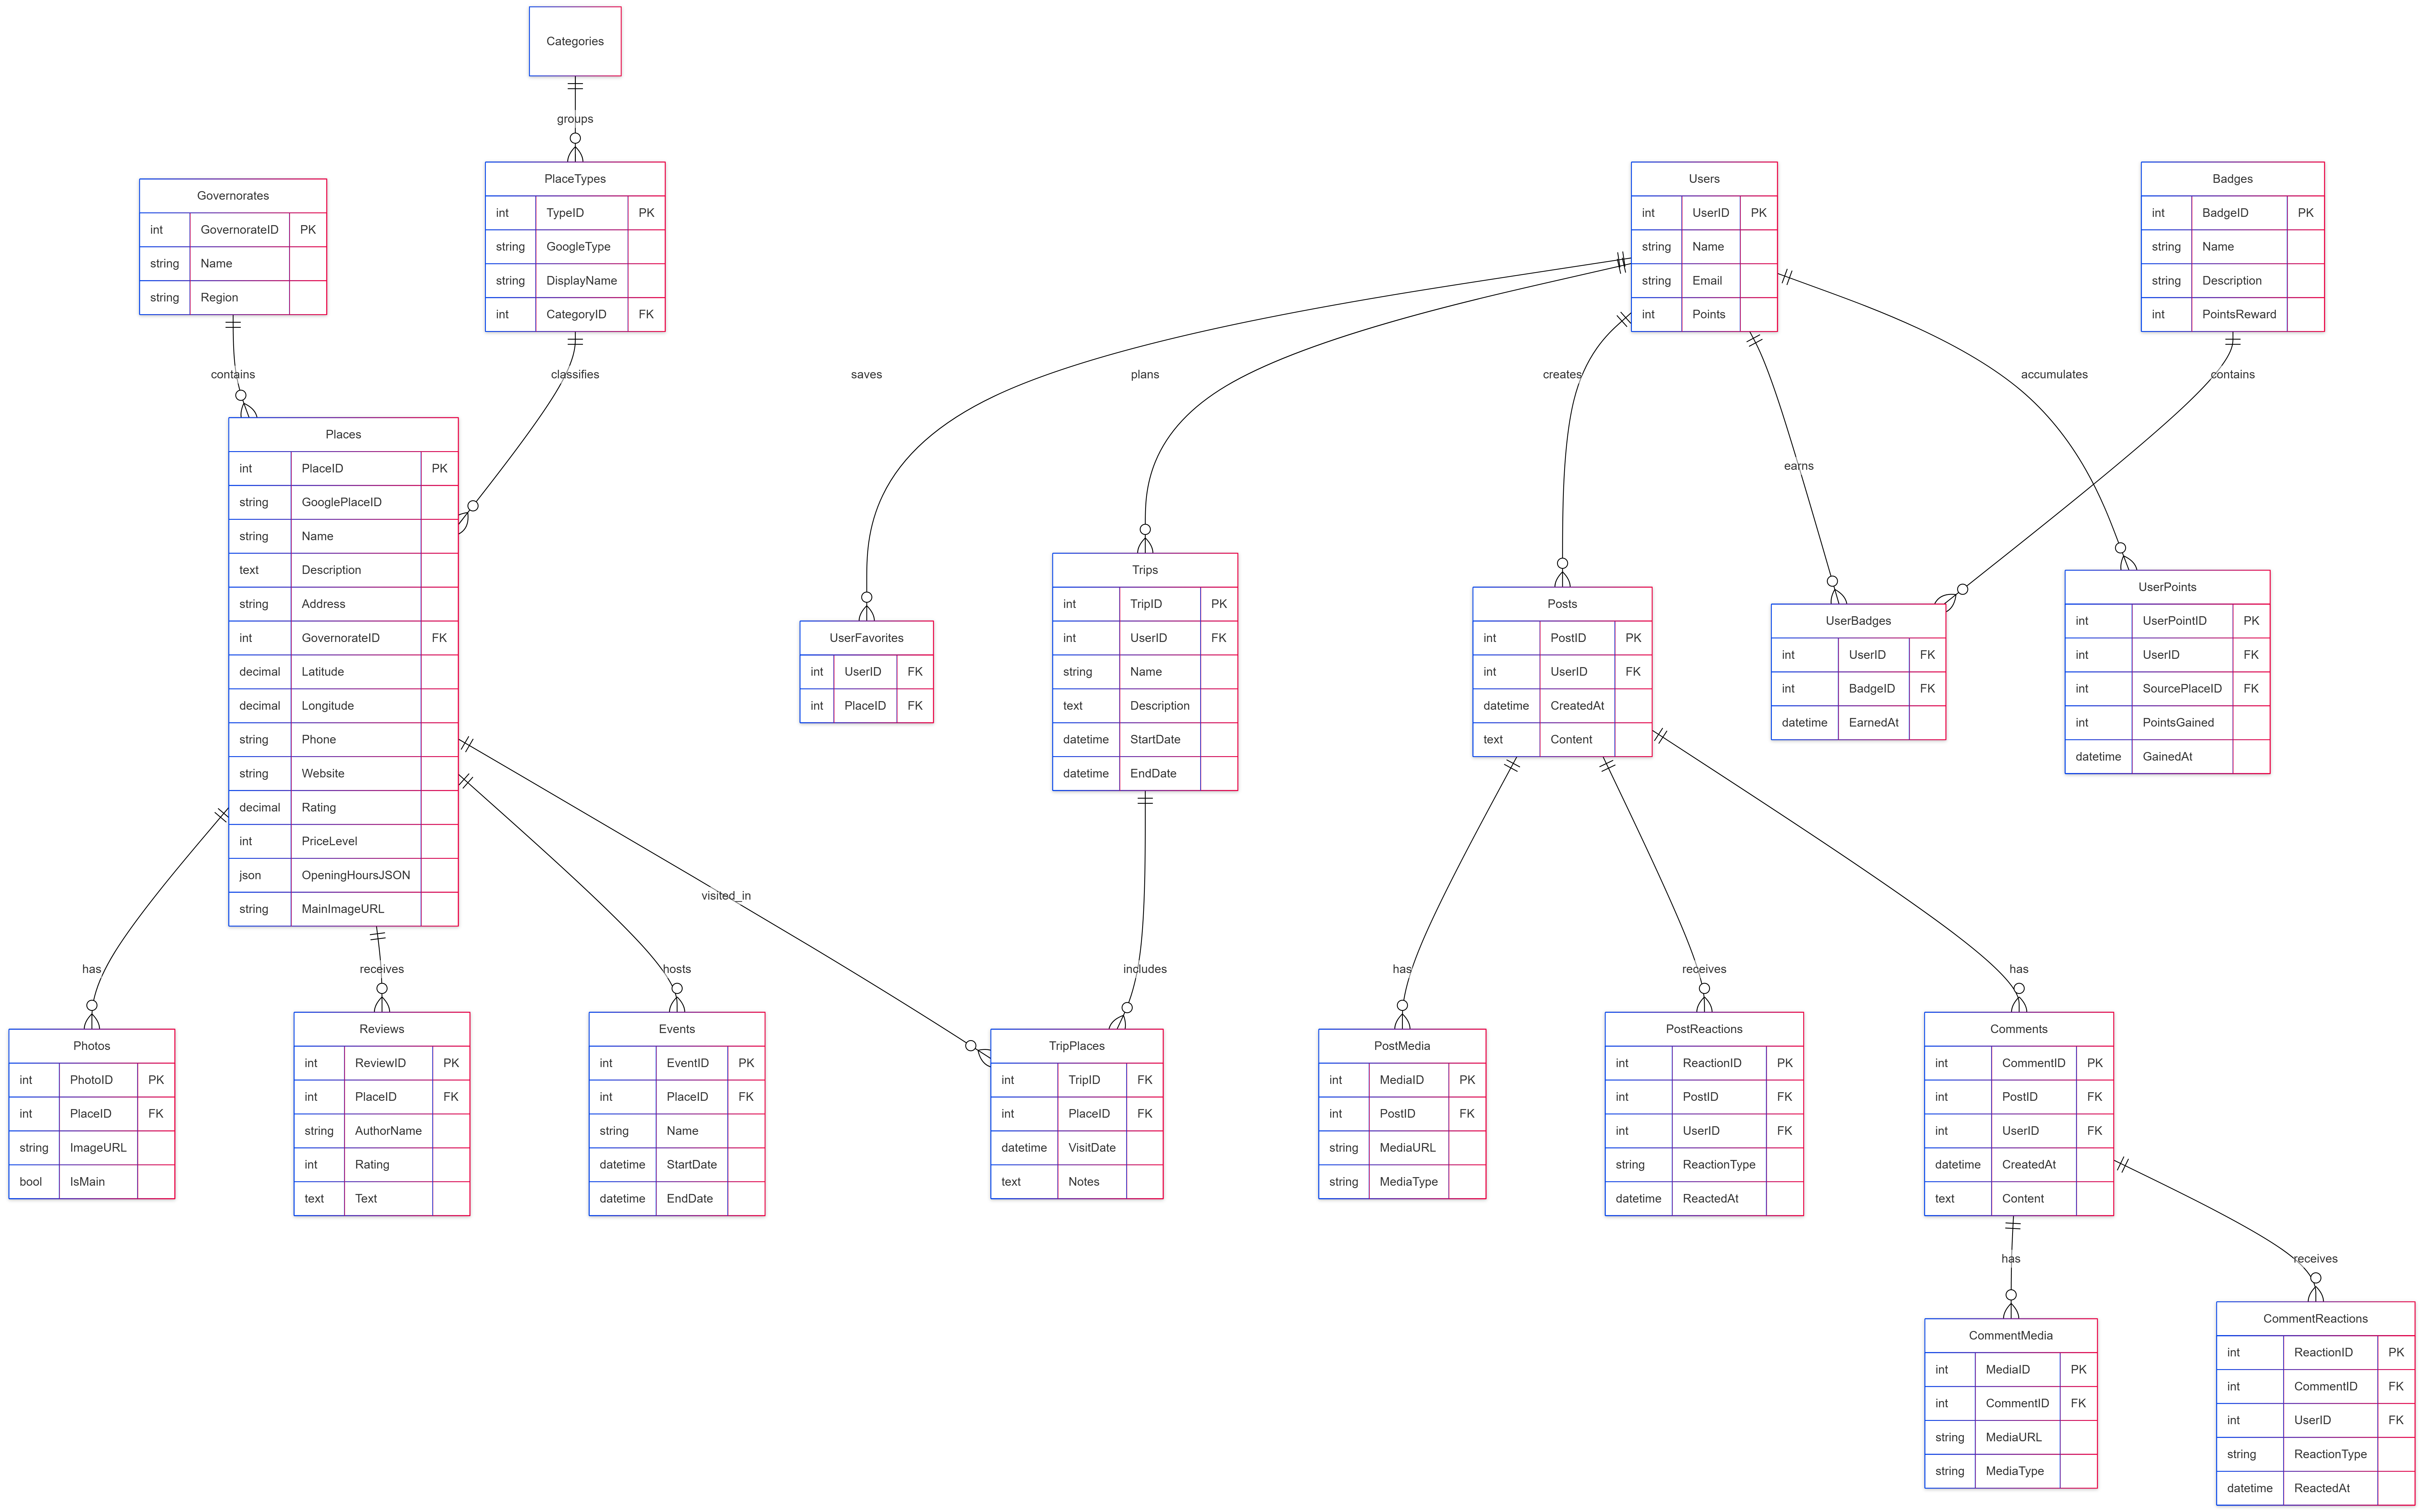
\includegraphics[width=\textwidth]{figures/erd.png}
    \caption{Kemora Full Database Entity Relationship Diagram}
    \label{fig:appendix_erd}
\end{figure}
